\documentclass[oneside,english]{amsart}
\usepackage{bbold}
\usepackage[T1]{fontenc}
\usepackage{inputenc}
\setlength{\parskip}{\smallskipamount}
\setlength{\parindent}{0pt}
\usepackage{amstext}
\usepackage{amsthm}
\usepackage{amsmath}
\usepackage{amssymb}
\usepackage{graphicx}
\usepackage{multirow}

\makeatletter
\numberwithin{equation}{section}
\numberwithin{figure}{section}
\theoremstyle{plain}
\newtheorem{thm}{\protect\theoremname}
\theoremstyle{definition}
\newtheorem{defn}[thm]{\protect\definitionname}
\theoremstyle{plain}
\newtheorem{prop}[thm]{\protect\propositionname}
\theoremstyle{remark}
\newtheorem{rem}[thm]{\protect\remarkname}
\theoremstyle{plain}
\newtheorem{lem}[thm]{\protect\lemmaname}
\theoremstyle{definition}
\newtheorem{example}[thm]{\protect\examplename}
\newtheorem{cor}[thm]{\protect\corollaryname}
\theoremstyle{definition}

\makeatother

\usepackage{babel}
\providecommand{\definitionname}{Definition}
\providecommand{\lemmaname}{Lemma}
\providecommand{\propositionname}{Proposition}
\providecommand{\remarkname}{Remark}
\providecommand{\theoremname}{Theorem}
\providecommand{\examplename}{Example}
\providecommand{\corollaryname}{Corollary}

\begin{document}
\title{Soft-Margin Tropical Support Vector Machines}
\author{Samuel Boïté, Théo Molfessis, Stéphane Gaubert, Xavier Allamigeon}
\begin{abstract}
We explore the novel application of tropical geometry to the realm of classification problems, specifically through the development of soft-margin Tropical Support Vector Machines. By leveraging the structural properties of the tropical semifield, we extend traditional linear classification methods into the tropical domain. We introduce Shapley operators to describe the convex hulls of data points, providing a geometrical approach for handling overlapping data using tropical projections. We then formulate a pseudo-polynomial algorithm to compute optimal-margin separating tropical hyperplanes. We extend this framework to handle multiple classes at once, showcasing its versatility and potential for various classification tasks. Finally, we introduce the 'kernel trick' in the tropical setting, mapping data points to higher-dimensional spaces through Veronese embeddings. Using tropically polynomial separation surfaces, we emulate neural network structures and offer a promising avenue for complex classification tasks. We present a proof of concept through empirical studies on standard datasets, highlighting the strengths and potential of tropical geometry in machine learning.
\end{abstract}

\maketitle


\section{Introduction}

The tropical semifield $\mathbb{R}_{\max}$ is the set of real numbers,
completed by $-\infty$ and equipped with the addition $a\oplus b=\max(a,b)$
and the multiplication $a\odot b=a+b$. 

\textbf{The tropical classification problem. }Given a set $\mathcal{I}$
of $d$-dimensional data points $x_{i}$ with associated labels $y_{i}\in\{\pm1\}$,
we define the classes $C^{+}$ (resp. $C^{-}$), consisting of the
points with positive (resp. negative) labels. We want to separate
our point clouds by a tropical hyperplane. We will extend this framework to $d$ classes of points later.


\begin{defn}
A \emph{tropical hyperplane of apex $u\in\mathbb{R}_{\text{max}}^{d}$
}splits $\mathbb{R}_{\max}^{d}$ depending on where $(x-u)$ reaches
its maximum coordinate:
\[
H_{u}:=\left\{ x\in\mathbb{R}_{\max}^{d},\quad(x-u)\,\text{reaches its max coordinate at least twice}\right\} .
\]

Such an hyperplane splits the space in $d$ different \emph{tropical
sectors}, depending on the coordinate maximized. A \emph{tropical
halfspace} of configuration $I\subset[d]$ is the union of tropical
sectors specified in $I$.

The \emph{signed tropical hyperplane }of configuration $I$\emph{
}is the surface between two complementary tropical halfspaces:
\[
H_{u}^{I}:=\left\{ x\in\mathbb{R}_{\max}^{d},\quad(x-u)\,\text{reaches its max coordinate in}\,I\,\text{and}\,I^{c}\right\} .
\]
\end{defn}

\begin{figure}[h]
\label{fig:(ex)}
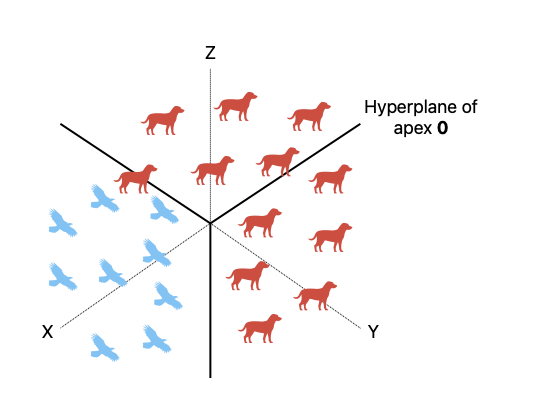
\includegraphics[scale=0.5]{fig/classification.png}
\caption{Binary classification problem}
\end{figure}

\section{Preliminaries}

\subsection{General setting}

The tropical binary classification problem itself is, as we will see, a subproblem of a more general one involving the notion of Shapley operators.

\begin{defn}
A \emph{Shapley operator} on $\mathbb{R}_{\max}$ is a map $T:\mathbb{R}_{\max}^{d}\longrightarrow\mathbb{R}_{\max}^{p}$
such that $T$ is non-decreasing and that for all $x\in\mathbb{R}_{\max}^{n}$
and $\lambda\in\mathbb{R}_{\max}$, $T(\lambda + x)=\lambda + T(x)$.

$T$ is said to be \emph{non-expansive }if it is $1$-Lipschitz.
\end{defn}

\begin{defn}
 An order-preserving and additively homogeneous self-map $F$ of
$\mathbb{R}_{\max}$ is said to be \emph{diagonal free} when $F_i(x)$ is independent of $x_i$ for all $i \in [n]$. In
other words, F is \emph{diagonal free} if for all $i \in [n]$, and for all $x,y \in \mathbb{R}_{\max}$ such that
$x_j = y_j$ for all $j \neq i$, we have $F_i(x) = F_i(y)$.   
\end{defn}


Let $T^\pm$ be two non-expansive Shapley operators. We define $$V^\pm = \{x\in\mathbb{R}^d,\quad x\le T^\pm(x)\},$$ which we want to separate with a tropical signed hyperplane.

\begin{defn}
For all $u\in\mathbb{R}_{\max}^{d}$, we define the \emph{tropical
norm} of $u$ as the largest difference between two of its coordinates:
\[
\lVert u\rVert:=\max u-\min u.
\]
The \emph{tropical distance} between $u$ and $v$ in $\mathbb{R}_{\max}^{d}$
is then defined as:
\[
d(u,v):=\lVert u-v\rVert.
\]
\end{defn}

\begin{defn}
$H_{u}^{I}$ is said to \emph{separate $V^{+}$ and $V^{-}$ with
a margin of at least} $\nu\ge0$ when:
\begin{enumerate}
\item $V^{+}$ and $V^{-}$ are respectively on either side of the hyperplane
$H_{u}^{I}$, i.e.
\[
\forall x\in V^{+},\qquad\text{argmax}_{i\in[d]}x_{i}\in I,
\]
\[
\forall y\in V^{-},\qquad\text{argmax}_{i\in[d]}x_{i}\in I^{c},
\]
or vice-versa.
\item Distance from $H_{u}^{I}$ to $V^{\pm}$ is at least $\nu$.
\end{enumerate}
When $\nu$ is maximal in the previous definition, we say that $H_{u}^{I}$
\emph{separates} $V^{\pm}$ \emph{with a margin of} $\nu$. When $\nu$
is zero, we say that $H_{u}^{I}$ \emph{separates} $V^{\pm}$.
\end{defn}

\subsection{Application to tropical convex hulls}

We shall see in this section that tropical projections are the right Shapley operator for describing and separating finite point clouds.

\begin{defn}
We define the \emph{tropical span} of a finite set of points $A=[a_{1}|\ldots|a_{p}]\in\mathbb{R}_{\max}^{d\times p}$
as the set of tropical linear combinations of these points:
\[
\text{Span}(A):=\left\{ A\odot\Lambda:=\lambda_{1}\odot a_{1}\oplus\cdots\oplus\lambda_{p}\odot a_{p},\quad\Lambda:=(\lambda_{i})_{i\in[p]}\in\mathbb{R}^{p}\right\} .
\]
Given the tropical convexity of these, these spans are often called
\emph{tropically convex hulls}, meaning the smallest tropically convex
sets containing them.
\end{defn}

\begin{defn}
Let $V$ a tropically convex, compact and nonempty subset of $\mathbb{R}_{\max}^{d}$.
We define the \emph{projection} of $x$ on $V$ as:
\[
P_{V}(x):=\max\{y\in V,\quad y\le x\}.
\]
When $V=\text{Span}(C)$ with $C$ in $\mathbb{R}_{\max}^{d\times p}$,
we will write the projection as $P_{C}$.
\end{defn}

The following property is derived by simple inequalities on $P_{C}$'s
expression with $\min$ and $\max$:
\begin{prop}
\label{prop:(Nondecreasing)}Let $C\in\mathbb{R}_{\max}^{d\times p}$.
$P_{C}$ is nondecreasing and for $x\in \mathbb{R}^d_\text{max}$, $P_{C}(x)\le x$.
\end{prop}

\begin{prop} (Formula 5.2.3 in \cite{Maclagan2015})
We have the following equality:
\[
P_{C}=CC^{\#},
\]
where for $i\in[d]$, $j\in[p]$ and $(x,z)\in\mathbb{R}_{\max}^{d}\times\mathbb{R}_{\max}^{p}$:
\begin{align*}
(Cz)_{i} & :=\max_{j\in[p]}\{C_{ij}+z_{j}\}\\
(C^{\#}x)_{j} & :=\min_{i\in[d]}\{-C_{ij}+x_{i}\}
\end{align*}
with the convention that $-(-\infty)+(-\infty)=-\infty$.
\end{prop}

\begin{rem}
Tropical projections are closely tied to mean payoff games. With $A$
and $B$ in $\mathbb{R}_{\max}^{p\times n}$, and $T=A^{\#}B$:
\[
\forall i\in[n],\quad T_{i}(x)=\min_{j\in[p]}\left\{ -A_{ji}+\max_{k\in[n]}(B_{jk}+x_{k})\right\} .
\]
In particular, $T_{i}(0)$ is the payoff, recieved by player MAX,
of one round of a zero-sum game with perfect information, where player
MIN starts from their state $i$, transitions to their opponent MAX's
state $j$ by receiving $A_{ji}$, who in turn chooses a MIN state
$k$ by recieving $B_{jk}$.

Therefore, $(T^{m}(0))_{i}$ is the \emph{value} of such a game after
$m$ consecutive rounds, having started in the MIN state $i$. The\emph{
escape rate }of the game defined by $T$ is defined by:
\[
\chi_{T}:=\lim_{m\rightarrow+\infty}\frac{T^{m}(0)}{m}.
\]
It is well known that this limit does exist and coincides with the \emph{mean payoff} of the game \cite{Allamigeon2018}. Under certain conditions, $\chi_{T}$ is the unique eigenvalue of the Shapley operator $T$.
\end{rem}

Let $P^\pm$ the projections associated with finite point clouds $C^\pm$. 

Operators $P^{\pm}$ can be slightly tweaked to make them \emph{diagonal-free}
(DF), a good property that will be of interest to us in the future.
In the modified game, the MIN player is prevented from replying to
his opponent eye-for-an-eye:
\[
\left[P_{\text{DF}}^{\pm}\right]:=\max_{j\in[p]}\left\{ C_{ij}^{\pm}+\min_{k\ne i}(-C_{kj}^{\pm}+v_{k})\right\}.
\]

\begin{prop}
$P^\pm_{\text{DF}}$ are diagonal-free Shapley operators that equivalently
describe $V^{\pm}$.
\end{prop}


\section{Separating finite overlapping data}

Assuming that the data overlap, we want to transform $V^{\pm}$ slightly
so as to make them separable by a tropical hyperplane.

\subsection{Measuring data overlap}
\begin{lem}
Intersection between convex hulls can be described using the Shapley operator:
\[
V^{+}\cap V^{-}=\left\{ v\in\mathbb{R}_{\max}^{d},\quad v\le T(v)\right\} ,
\]
where $T = T^+\wedge T^-$.
\end{lem}

As we have a Shapley operator, the analogy with game theory applies, and the notions of Collatz-Wielandt numbers, spectral radus and game value are identical \cite{AKIAN2012}. We can then state the following theorem:
\begin{thm}
(Allamigeon, Gaubert et al. \cite{Allamigeon2018}) $V^{+}\cap V^{-}$
contains a Hilbert ball of positive radius if and only if the spectral
radius of $F$, defined as
\[
\rho(T)=\sup\{\mu\in\mathbb{R},\quad\exists z\in\mathbb{R}^{d},\quad T(z)=\mu + z\}
\]
is strictly positive. In this case, $\rho(F)$ is the inner radius
$\text{inrad}(V^{+}\cap V^{-})$, i.e supremum of the radii of the
Hilbert balls contained in it.
\end{thm}

We can then apply the following algorithm to compute the eigenpair
in pseudo-polynomial time.

\subsection{Efficiently finding the eigenpair}

We now describe the following projective Krasnoselskii-Mann iteration
algorithm. Given an initial point
$a^{0}$, we iteratively compute:
\[
\begin{cases}
z^{k+1} & =\frac{a^{k}+T(a^{k})}{2}\\
a^{k+1} & =z^{k+1}-\max_{i\in[d]}z_{i}^{k+1}\cdot\textbf{1}_{d}
\end{cases}
\]

The following convergence theorem follows from \cite{Cominetti2013}.
\begin{cor}
As $T$ is a non-expansive Shapley operator, the Krasnoselskii-Mann
algorithm converges in pseudo-polynomial time.
\end{cor}

The eigenpair we search is $\left(a^{\infty},2\cdot\max_{i\in[d]}z_{i}^{\infty}\right)$.

\subsection{Separating overlapping finite data}
We place ourselves in the case of separation of finite tropical convex envelopes. We have seen that the corresponding Shapley operator is the diagonal-free operator.

We now define a process for separating overlapping data. Assuming
$V^{+}\cap V^{-}\ne\emptyset$, let $\left(a,\lambda\right)$ the
eigenpair of $T$ approximated by the iteration algorithm.
\begin{prop}
For all sector $i \in [d]$, we choose one class $\pm_i$ such that 

$T(a)_i = T^{\pm_i}(a)_i = \lambda + a_i,$ (we note $\mp_i$ the other one)  and we project all points of $C^{\pm_i}$ located in sector $i$ onto $H_{a}$. Then the intersection
of new convex hulls $W^{\pm}$ is of empty interior.
\end{prop}


\begin{proof}
Let $Q^{\pm}$ be the \emph{diagonal-free} operators over transformed point clouds, and $Q = Q^+ \wedge Q^-.$ We prove that $Q(a) = a$. We use the following notations for $j\in [p]$:
$$\begin{gathered}
\begin{aligned}
& \left\{
\begin{array}{l}
D^{\pm}_{ij} := C_{ij}^{\pm} - a_i  \\
m_{kj}^{\pm} := W^{\pm}_{kj} - a_k \\
c^{\pm}_{ij} :=  W^{\pm}_{ij} - \max_{k\ne i} m^{\pm}_{kj}
\end{array}
\right.
\end{aligned}
\end{gathered}$$

We also write $s^\pm(j)$ the sector of $C^\pm_{\cdot j}$, and $d^\pm(j)$ the second argmax of $D^\pm_{\cdot j}$.

The transformation defined above consists in setting $W^{\pm_i}_{ij} = C^{\pm_i}_{ij} - \mathbb{1}_{i= s^{\pm_i}(j)} \cdot d(C^{\pm_i}_{\cdot j}, H_a)$ and $W^{\mp_i}_{ij} = C^{\mp_i}_{ij}$. It leads by construction to $m_{s^{\pm}(j)j}^{\pm} \geq D^{\pm}_{d^{\pm}(j)j}$  with equality if the class of $C^\pm_{\cdot j}$ is the one chosen in its sector, which can be noted  $\pm = \pm_{s^{\pm}(j)}$.



We can also write that $Q^{\pm}(a)_i = \max_{j \in [p]} c^{\pm}_{ij}.$



Let $i\in [d]$. If $C^{\pm}_{\cdot, j}$ isn't in the $i$-th sector, then for $k \neq s^{\pm}(j) $, we have $m_{kj}^\pm \leq D^{\pm}_{d^{\pm}(j)j} \leq m_{s^{\pm}(j)j}^{\pm}$. Therefore, in that case, $c^{\pm}_{ij} = D^{\pm}_{ij} - m_{s^{\pm}(j)j}^{\pm} + a_i \leq a_i.$

Otherwise, $s^{\pm}(j) = i $ and $\max_{k\ne i} m^{\pm}_{kj} = D^{\pm}_{d^{\pm}(j)j}$, thus $c^{\pm}_{ij} =   m_{s^{\pm}(j)j}^{\pm} - D^{\pm}_{d^{\pm}(j)j}+ a_{s^{\pm}(j)} \geq a_{s^{\pm}(j)} = a_i, $
with equality if $\pm = \pm_{s^{\pm}(j)}$.


Lastly, using the proof of Theorem 22 in \cite{Akian2021TropicalLR}, we know that there exists $j^{\pm_i}, j^{\mp_i}\in [p]$ such that $C^{\pm}_{\cdot j^{\pm}}$ are in sector $i$. Therefore, $c_{ij^{\pm_i}}^{\pm_i} = a_i$ and $c_{ij^{\mp_i}}^{\mp_i} \geq a_i$. Hence
$Q(a)_i= Q^{\pm_i}(a)_i = a_i$, and finally $Q(a)=a$.


\end{proof}
\begin{example}
Here is what the transformation yields with a toy inseparable dataset:

\begin{figure}[!h]
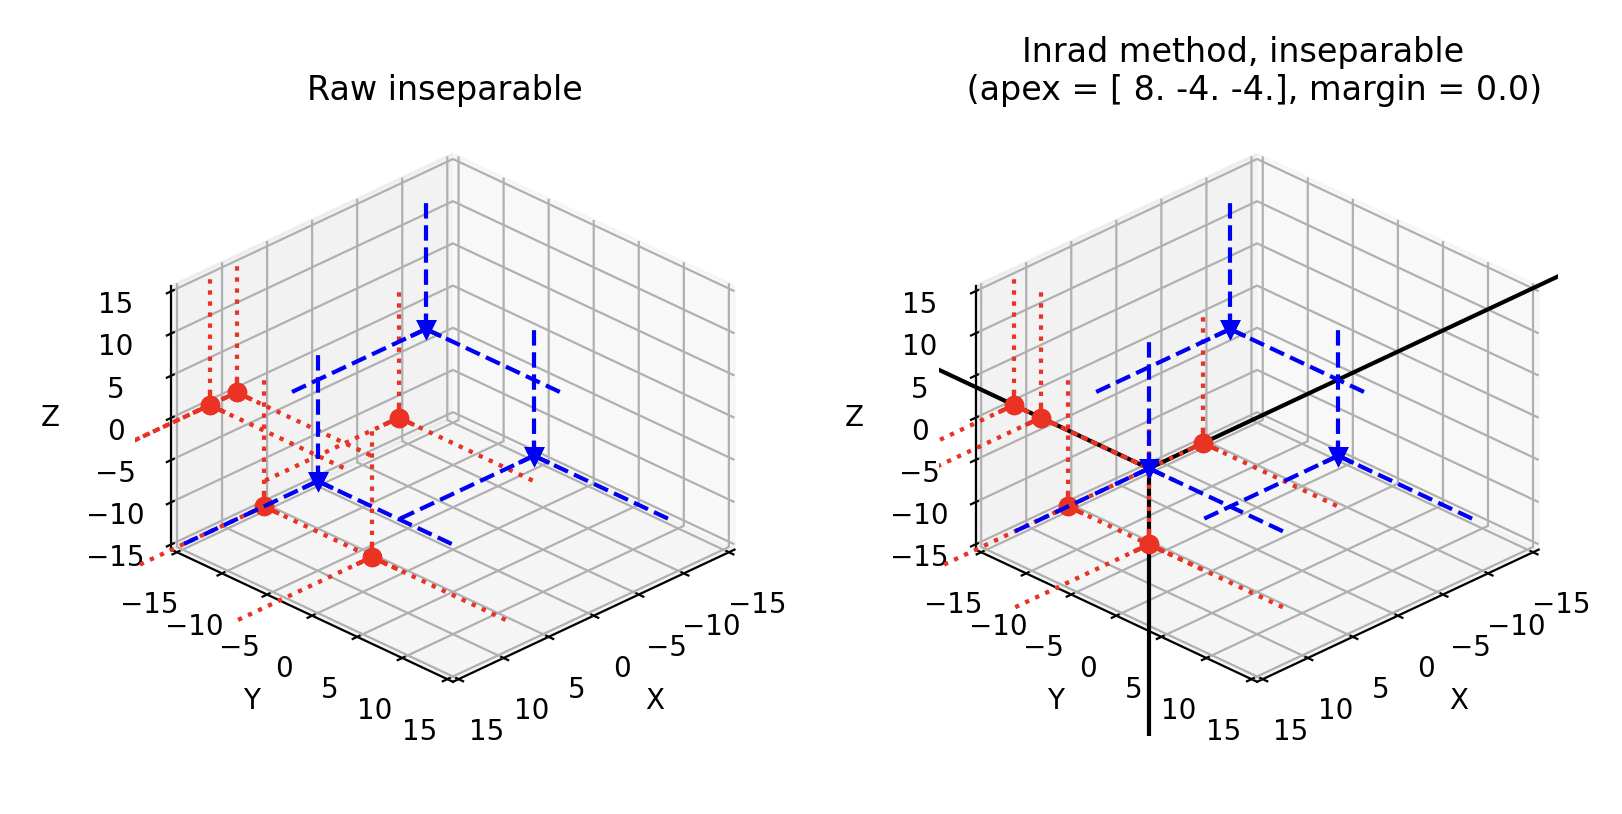
\includegraphics[scale=0.4]{fig/inseparable.png}
\caption{Separating convex hulls}
\end{figure}
\end{example}

\begin{rem}
We would have to deal with the
branching points that don't contribute to increasing the interior of the intersection. 
\end{rem}


\section{Optimal-margin separating hyperplanes}

Assuming that data is now separable, we prove that the previous
method can be extended to give us separating hyperplanes with maximal
margin.
\begin{rem}
When $V^{+}$ and $V^{-}$ are disjoint, the spectral radius $\lambda$
of $T$ is strictly negative. From \cite{AKIAN2021}, we may see
$-\lambda$ as the eigenvalue an operator $T^{\text{dual}}$
in dual space, as $T$ is itself a finitely-generated
Shapley operator. This would give us a complementary inner radius
interpretation, and makes $H_{a}$ a great candidate in the separable
case.
\end{rem}

Let $(a,\lambda)$ the eigenpair of $T$ approximated
by previous algorithm, verifying $T(a)=\lambda+a$. Let's define the sectors:
\[
I^{\pm}:=\{i\in[d],\quad T^{\pm}(a)_{i}>\lambda+a_{i}\}.
\]

\begin{prop}
$H_{a}^{I}$, given the sectors defined above, separates $V^{+}$ and
$V^{-}$ with a margin of $-\lambda$. Moreover, this margin is optimal in the case where $T^{\pm}$ are of the form $T^{\pm}(x) = P_{V^{\pm}}(x) = \sup_{v\in V^{\pm}} \left( v_i + \min (-v + x)\right),$ which is in particular the case when separating finite point clouds.
\end{prop}

\begin{proof}
As $T^\pm$ is non-expansive, let's first remark that for  $x^\pm\in V^\pm$:
$$x^\pm_i  \le T^{\pm}(x^\pm)_{i} =\left(T^{\pm}(x^\pm)-T^{\pm}(a)\right)_{i}+T^{\pm}(a)_{i},$$
hence
\begin{equation}\label{eq41}
x^\pm_i \le\max(x^\pm-a)+T^{\pm}(a)_{i}.
\end{equation}
For instance, let $i\in [d] \setminus I^{+}$.
Then $T^{+}(a)_{i}=\lambda+a_{i}$,
so for $x^{+}\in V^{+}$, using equation \ref{eq41}:


\[
x_{i}^{+}-a_{i}\le\max(x^+-a)+\lambda.
\]

In particular, $x^+_i-a_i < \max(x^+-a)$ and any element of $V^+$ can't belong to any of sectors in $[d] \setminus I^{+}$ with respect to $H_a$, from which the sectors $I^\pm$ are well-defined. Finally,
\[
d(H_{a}^{I},x^+)=\max(x^+-a)-\max(x^+-a)_{[d] \setminus I^{+}}\ge-\lambda,
\]
and the margin comes from the fact that this applies to any element of $V^+$. 

Let's finally prove that the margin is maximal in the case where $T^{\pm}$ are of the form $T^{\pm}(x) = P_{V^{\pm}}(x) = \sup_{v\in V^{\pm}} \left( v_i + \min (-v + x)\right).$ Let $i\in [d] \setminus I^{+}$. Then, for $\varepsilon > 0$, we can find $v \in V^+$ such that $$ T^+(a)_i - \varepsilon \le v_i - \max(v - a) \le T^+(a)_i,$$ giving us $$\lambda - \varepsilon \le v_i - a_i - \max(v - a) \le \lambda.$$ Maximizing over all $i\in [d] \setminus I^{+}$ yields that $v$ is at most at distance $-\lambda + \varepsilon$ of $H_a^I$, hence the optimality.


\end{proof}
\begin{example}
Here is what the algorithm gives with a toy separable dataset:

\begin{figure}[!h]
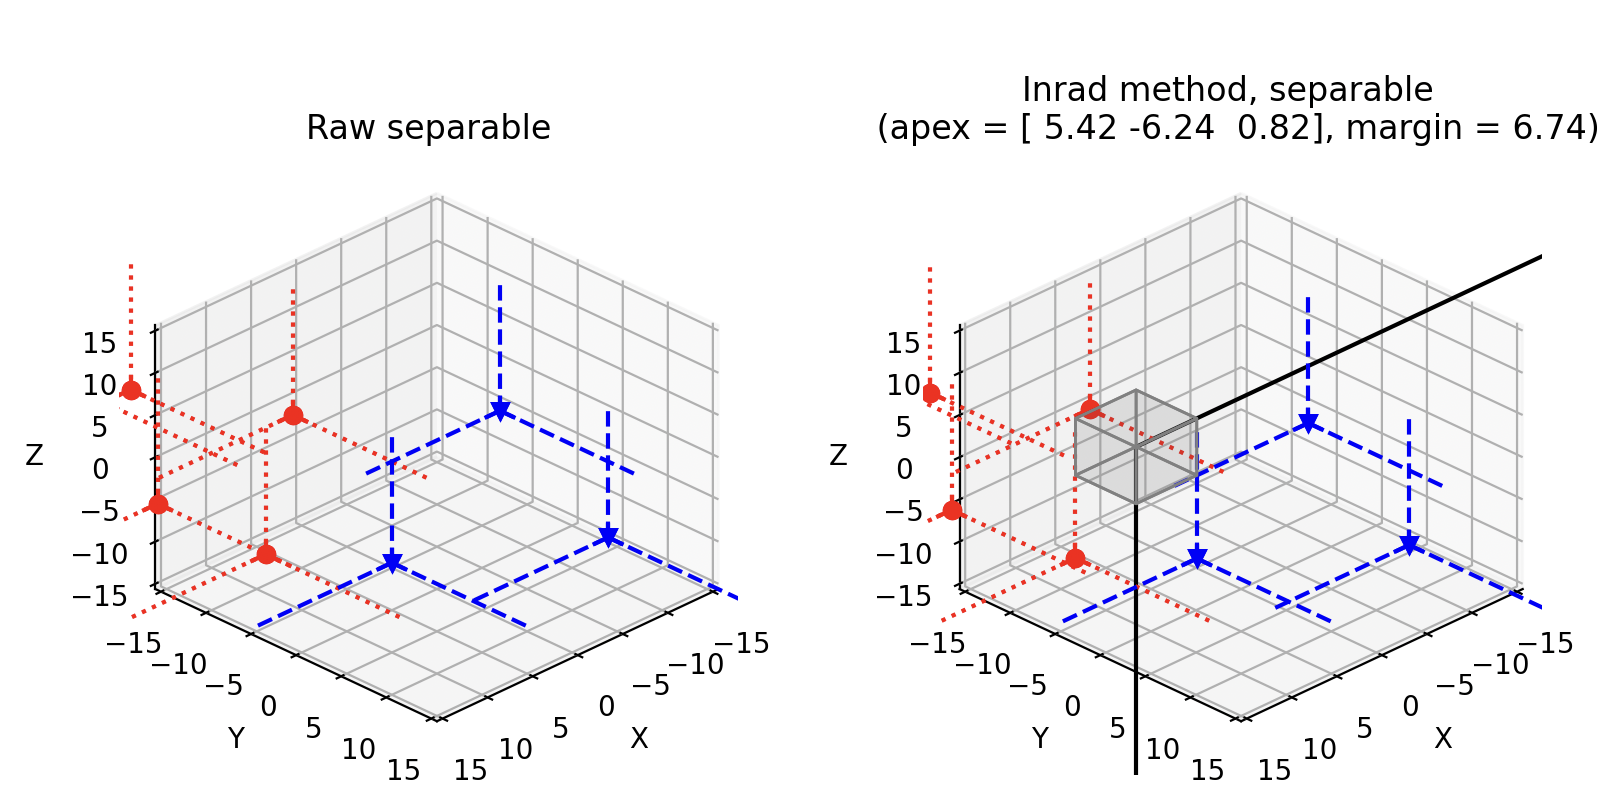
\includegraphics[scale=0.45]{fig/separable.png}
\caption{Optimal-margin separable hyperplane}
\end{figure}
\end{example}

\section{Multi-class optimal-margin separation}

In this section, we consider convex hulls of point clouds of $D$ classes, noted $V^k$ for $k\in [D]$, and described by Shapley operators $T^k$. We give a sufficient condition for these classes to be tropically separable in their whole, meaning that there exists a tropical signed hyperplane such that each $V^k$ belong to sectors of $I^k \subset [d]$ with $I^k\cap I^l = \emptyset$ for $k\ne l \in [D].$
We then adapt the previous results to this case.


We now consider the Shapley operator :

$$T := \bigvee_{1\le k < l \le D} T^k \wedge T^l$$

We remark that in the case $D=2$, $T$ is the same as previously defined.

Let $(a,\lambda)$ the eigenpair of $T$ approximated
by the Kranoselskii-Mann algorithm, verifying $T(a)=\lambda+a$. Let's define the sectors:
\[
I^{k}:=\{i\in[d],\quad T^{k}(a)_{i}>\lambda+a_{i}\}.
\]

Given the definition of $T$, it is clear that $I^k\cap I^l = \emptyset$ for $k\ne l \in [D],$ and we have the following result :

\begin{prop}
If $\lambda < 0$, the signed tropical hyperplane $H_{a}^{I}$, given the sectors defined above, separates $V^{k}$ and
$V^{l}$ for all $k\ne l \in [D]$ with a margin of $-\lambda$. Moreover, this margin is optimal in the case where all $T^{k}$ are of the form

$T^{k}(x) = P_{V^{k}}(x) = \sup_{v\in V^{k}} \left( v_i + \min (-v + x)\right),$ which is in particular the case when separating finite point clouds.
\end{prop}

\begin{proof}
    Let $k\in [D]$ and $i \in [d] \setminus I_k$. Using the same reasoning as in the proof of Proposition $19$, we obtain that for all $x^k \in V^k$,  $$d(H_{a}^{I}, x^k) =\max(x^k-a)-\max(x^k-a)_{[d] \setminus I_k} \ge-\lambda,$$ hence the margin. Let's now prove the optimality in the case where all $T^{k}$ are of the form $T^{k}(x) = P_{V^{k}}(x) = \sup_{v\in V^{k}} \left( v_i + \min (-v + x)\right).$ For all $i\in [d]$, there are two distinct classes $k \ne l \in [D]$ such that $T^{k}(a)_i\wedge T^{l}(a)_i = \lambda +a_i$. As $I^k\cap I^l = \emptyset$, we can suppose by symmetry that $i \in [d]\setminus I_k.$ Then using the same argument as in the proof of optimality in Proposition $19$, we know that for all $\varepsilon > 0$ there is a point $v^k \in V^k$ such that $\max(v^k-a)-(v^k_i-a_i) \le - \lambda + \varepsilon$, which means that $$d(H_{a}^{I}, x^k) =\max(x^k-a)-\max(x^k-a)_{[d] \setminus I_k} \le -\lambda + \varepsilon.$$

    As this holds for every sector $i\in [d]$, we have proven the optimality. (???)
\end{proof}

\section{Kernel trick: tropically polynomial decision boundaries}

In the classical setting, the kernel trick consists in mapping the training points in a higher-dimensional space in which we expect the data to become easily linearly separable. In this paragraph, we generalize this idea to integer combinations of features in the tropical setting. 

If $\mathcal{A}\subset \mathbb{Z}^d$ is a set of vectors, we define the \emph{veronese embedding} of $x$ as $$\text{ver}(x) = \left(\langle x, \alpha \rangle\right)_{\alpha\in \mathcal{A}}\in\mathbb{R}^\mathcal{A},$$ allowing us to map our point space into a larger space, made up of various integer combinations of features. Noting $s\in\mathbb{N}$ a scale parameter, and $\Delta_d$ the $d$-dimensional simplex, we take $$\mathcal{A}_s := (s\Delta_d) \cap \mathbb{Z}^d.$$

\begin{prop}
Applying the previous method to point clouds $\text{ver}(C_i)$ for each class $i$ yields a classifier whose decision boundaries, when seen in the initial vector space, are tropical polynomials.
\end{prop}

Feedforward neural networks with rectified linear units are, modulo trivialities, nothing more than tropical rational maps \cite{zhang2018tropical}, i.e differences of tropical polynomials. Thus, the framework we have chosen is close to that of dense neural networks, and should yield similar results for classic datasets.

We therefore consider:
\begin{itemize}
    \item The \emph{Iris flower dataset}, which includes measurements such as sepal length, sepal width, petal length, and petal width, across three species of Iris (Iris setosa, Iris virginica, and Iris versicolor). This dataset is commonly used for classification tasks and testing clustering algorithms.
    \item The \emph{Breast Cancer Wisconsin dataset}, which contains features computed from a digitized image of a fine needle aspirate of a breast mass. The features describe characteristics of the cell nuclei present in the image, and the dataset is primarily used for binary classification tasks to distinguish between malignant and benign tumors.
    \item The \emph{Wine quality and type dataset}, which comprises physicochemical tests (like alcohol content, acidity, sugar level, etc.) and sensory information (quality score) for various samples of red and white wines. This dataset is often employed for regression tasks to predict wine quality or for classification tasks to differentiate between wine types.
    \item The \emph{FIFA 2022 cards dataset}, which includes skill ratings of players featured in the game and playing positions. This dataset can be used to predict positions on the field.
\end{itemize}

These datasets have the characteristic of having features that are comparable with each other, which makes them suitable for the tropical framework -- although this should work in any case with the kernel trick, since we're describing objects analogous to DNNs.

So as not to bother with branches in the non-separable case, we assign the sectors to the majority population, which in particular settles these borderline cases.

\begin{figure}[!h]
\begin{tabular}{|c|c|c|c|}
\hline 
Dataset & Groups & $d$ & $p$\tabularnewline
\hline 
\hline 
Iris & Setosa, Virginica, Versicolor & 4 & 150\tabularnewline
\hline 
Cancer & Malign, Benign & 31 & 570\tabularnewline
\hline 
Wine & Red (bad), Red (good), White (bad), White (good) & 10 & 6500\tabularnewline
\hline 
FIFA & Striker, Center back, Center mid, Goal & 34 & 19240\tabularnewline
\hline 
\end{tabular}


\caption{Datasets description}
\end{figure}

The sets $A_s$ grow exponentially with the dimension and polynomially with $s$, and encode the complexity of the mimicked neural network. $s$ will therefore be a relevant hyperparameter of overfitting or underfitting.

\begin{figure}[!h]
\begin{tabular}{|c|c|c|c|c|c|c|c|c|c|c|}
\hline 
\multirow{2}{*}{Dataset} & \multicolumn{2}{c|}{
Hyperplane} & \multicolumn{2}{c|}{$\mathcal{A}_{1}$} & \multicolumn{2}{c|}{$\mathcal{A}_{2}$} & \multicolumn{2}{c|}{$\mathcal{A}_{3}$} & \multicolumn{2}{c|}{$\mathcal{A}_{4}$}\tabularnewline
\cline{2-11} \cline{3-11} \cline{4-11} \cline{5-11} \cline{6-11} \cline{7-11} \cline{8-11} \cline{9-11} \cline{10-11} \cline{11-11} 
 & \emph{1v1} & \emph{1vR} & \emph{1v1} & \emph{1vR} & \emph{1v1} & \emph{1v1} & \emph{1v1} & \emph{1vR} & \emph{1v1} & \emph{1vR}\tabularnewline
\hline 
Iris & 70\% & 83\% & 70\% & 87\% & 93\% & 93\% & 90\% & 87\% & 87\% & 87\%\tabularnewline
\hline 
Cancer & 90\% & 89\% & 90\% & 89\% & 90\% & 91\% & 88\% & 86\% & $\cdots$ & $\cdots$\tabularnewline
\hline 
Wine & 67\% & 57\% & 67\% & 56\% & 72\% & 74\% & 78\% & 85\% & 87\% & 92\%\tabularnewline
\hline 
FIFA & 78\% & 69\% & 78\% & 69\% & 79\% & 77\% & $\cdots$ & $\cdots$ & $\cdots$ & $\cdots$\tabularnewline
\hline 
\end{tabular}

\caption{Accuracies for one-vs-one and one-vs-rest classifiers}
\end{figure}

In the table, the dots indicate overfitting, or that the dimension has become too large for the calculations to succeed.

The addition of complexity by our kernel method seems particularly effective for the wine dataset.

We note that irrelevant features are driven out of the decision process by a correspondingly large coordinate in the apex, preventing this feature from being maximal. This could guide us towards heuristics to remove superfluous features, combat overfitting and reduce training time.

\newpage
\bibliographystyle{plain}
\bibliography{ea}

\end{document}
